\section{Two-Level attention on BoSs Memory}
\label{ssec:hierarattn}

To visualize the benefit of two-level attention used on {\sc BoSs} memory by the decoder, we compare attention weights for two models: our proposed \emph{two-level attention} and a variant with just \emph{one-level attention} (over all the words in the memory). In the example of a sample dialog from bAbI Task 3, shown in Figure \ref{fig:attention}, the decoder is aimed at predicting the second best restaurant \textit{3 stars}, given that the restaurant with rating \textit{8 stars} has already been suggested and rejected. We show attention only on the KB entries for brevity.

The models share some similarities in their distribution of attention. First, the attention weights are localized over the restaurant names, indicating the preference of the system to point to a specific restaurant. This is supported by the $g_s$ values, $3.14$ x $10^{-5}$ and $1.15$ x $10^{-4}$ for two-level attention and one-level attention respectively, i.e., both models prefer to copy rather than generate. Moreover, entries with the same restaurant name have similar attention weights, reflecting the robustness of the distribution.

We also observe that two-level attention is able to perform the difficult task of {\em sorting} the restaurant entries based on decreasing order of rating (number of stars). It gives more weight to entries with a high rating 
(\textit{3 stars} $>$ \textit{2 stars} $>$ \textit{1 star})
and suppresses the weights of any previously suggested restaurant.
%, e.g., \textit{8 stars}. 

The attention over memory cells provides \sys\ with the ability to infer over multiple sets of tuples. The ability to sort the restaurants and reject a previously seen restaurant can be observed by the attention heat map of Memory cells. Attention over tokens on the other hand can push the attention weights towards either the subject or object in the KB tuple, based on the query's request. Thus using both in conjunction helps \sys\ perform significantly better than the baselines and illustrates the importance of the {\sc BoSs} memory in comparison to a flat memory layout.

\begin{figure*}
\centering
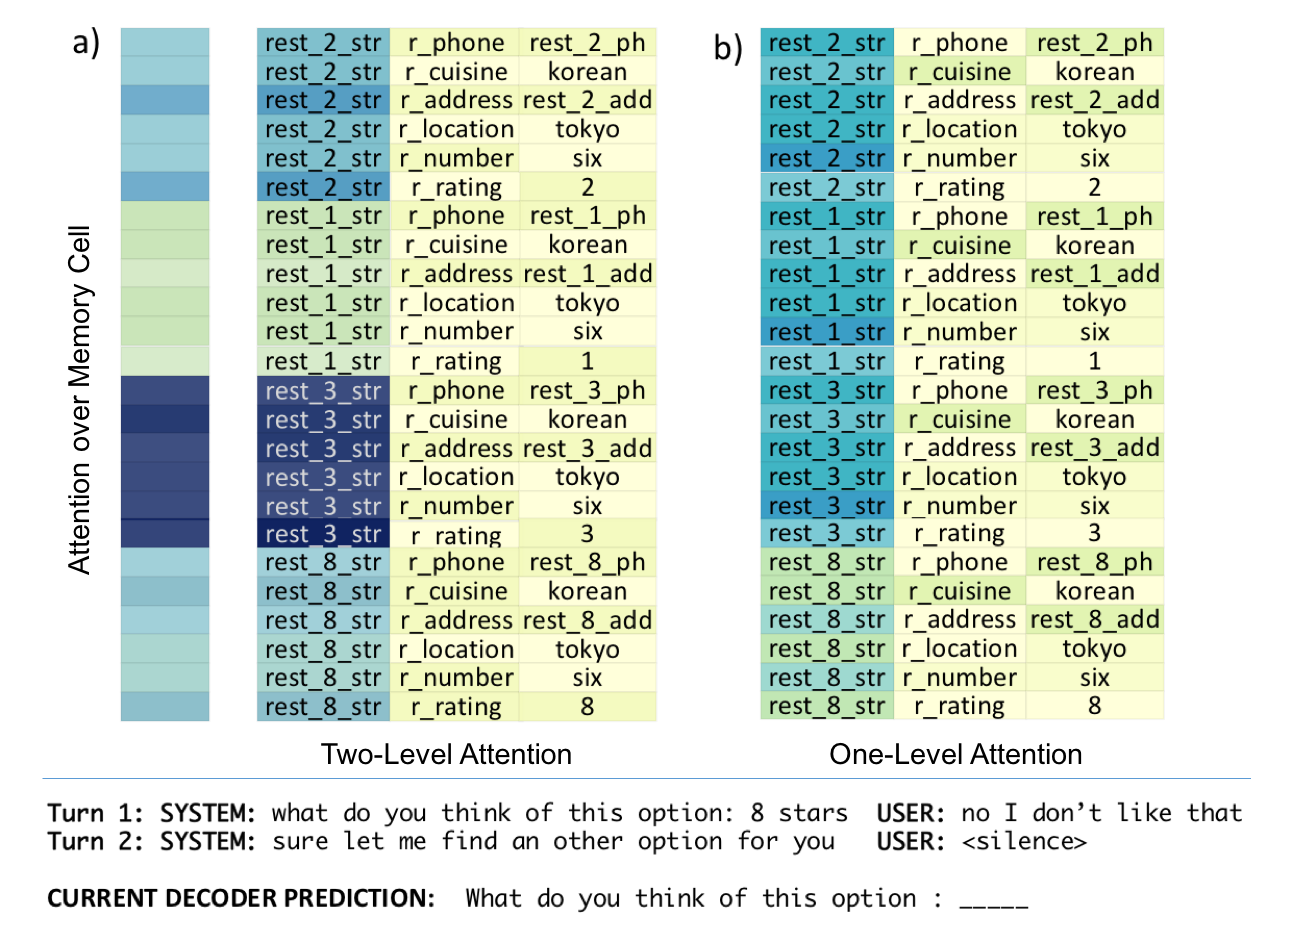
\includegraphics[width=0.8\textwidth]{assets/task3_two_level.png}
\caption{Visualization of attention weights on selected portions of memory in (a) \sys\ with two-level attention vs (b) \sys\ with one-level attention}
\label{fig:attention}
\end{figure*}

\section{Reproducibility}
\label{sec:reproduce}
We list out the complete set of hyperparameters used to train \sys\ for the various datasets in Table \ref{tab:params}. Our code will be made publicably accessible for future research purposes. Our trained models and evaluation scripts will also be provided. We will also make our end-to-end reconstruced Camrest dataset along with our whole batch of knowledge adaptability test sets available.

\begin{table*}[ht]
\centering
\footnotesize
\begin{tabular}{c|ccccc}
\toprule
\textbf{Task} & \textbf{Learning Rate} & \textbf{Hops} &  \textbf{Embedding Size} & \textbf{Disentangle Loss Weight} & \textbf{DLD}\\
\midrule
T1 & 0.001 & 1 & 128 & 1.0 & 0.2 \\
T2 & 0.001 & 1 & 128 & 1.0 & 0.2 \\
T3 & 0.0005 & 3 & 128 & 1.5 & 0.2 \\
T4 & 0.001 & 1 & 128 & 1.0 & 0.2 \\
T5 & 0.0005 & 3 & 256 & 1.0 & 0.2 \\
CamRest & 0.0005 & 6 & 256 & 1.0 & 0.2 \\
SMD & 0.0005 & 3 & 256 & 1.0 & 0.1 \\
\bottomrule 
\end{tabular}
\caption{The hyperparameters used to train \sys\ on the different datasets}. 
\label{tab:params}
\end{table*}

\section{Example Predictions of \sys\ and Baselines}
\label{sec:examples}
Examples from SMD is shown in Table \ref{tab:smd0} respectively. Examples from KA test set with percentage of unseen entites set to 50 from CamRest and SMD are shown in Table \ref{tab:cam50} and Table \ref{tab:smd50} respectively. Examples from KA test set with percentage of unseen entites set to 100 from bAbI dialog Task 1 is shown in Table \ref{tab:t1_100}.

\begin{table*}
\centering
\small
\begin{tabular}{c|l}

\toprule
% \multicolumn{2}{c}{\textbf{KB (restaurant|cuisine|address|phone|postcode)}} \\
% \multicolumn{2}{c}{\textit{prezzo}|\textit{ethiopian}|\textit{22\_seetharam\_nagar}|\textit{01799\_521260}|\textit{cb30ad}}\\
% \midrule
\midrule
\textbf{usr-1} &good morning \\
\textbf{sys-1} & hello what can i help you with today \\
\textbf{usr-2} & can you book a table with \textit{korean} cuisine for \textit{five} in \textit{beijing} \\
\textbf{sys-2} & i ' m on it . which price range are looking for ? \\
\textbf{usr-3} & i am looking for a \textit{overpriced} restaurant \\
\midrule
\textbf{Gold} & api\_call \textit{korean beijing five overpriced}
 \\
\midrule
\midrule
\specialcell[t]{\textbf{Seq2Seq+Copy}} & api\_call \textit{korean beijing five overpriced}
 \\
\midrule
\textbf{Seq2Seq} & api\_call \textit{french london four moderate} \\

\midrule
\textbf{Mem2Seq} & api\_call \textit{overpriced korean korean overpriced}
 \\
\midrule
\textbf{\sys\ } & api\_call \textit{korean beijing five overpriced} \\
\bottomrule
\end{tabular}
\caption{Example from bAbI dialog Task 1 with 100\% OOV.}
\label{tab:t1_100}
\end{table*}
\begin{table*}
\centering
\small
\begin{tabular}{c||p{13cm}}
\toprule
\multicolumn{2}{c}{\textbf{KB (restaurant|cuisine|address|phone|postcode)}} \\
\multicolumn{2}{c}{\textit{prezzo}|\textit{ethiopian}|\textit{22\_atlantis\_road}|\textit{01799\_521260}|\textit{cb30ad}}\\
\midrule
\midrule
\textbf{usr-1} &i want a \textit{moderately\_expensive ethiopian} restaurant in the \textit{south} side of town \\
\textbf{sys-1} & i ' m sorry . i can not find a \textit{moderately\_expensive ethiopian} restaurant in the \textit{south} side of town \\
\textbf{usr-2} & i would like to find a \textit{moderately} priced restaurant in the \textit{west} part of town \\
\textbf{sys-2} & \textit{prezzo} is a moderately priced \textit{ethiopian} restaurant in the \textit{west} part of town . there is also \textit{indian} and \textit{british} food available in that area and price range . would you like more info ? \\
\textbf{usr-3} & yes can i get thier address and postcode ? \\
\midrule
\textbf{Gold} & of course , \textit{prezzo} ' s address is \textit{22\_atlantis\_road} and postcode is \textit{cb30ad}
 \\
\midrule
\midrule
\specialcell[t]{\textbf{Seq2Seq+Copy}} & postcode a is is \textit{01223350688} UNK there get i for for today
 \\
\midrule
\textbf{Seq2Seq} & the address is \textit{83\_regent\_street} and their postcode is \textit{cb58aq} \\

\midrule
\textbf{Mem2Seq} & the phone address is \textit{cb21uj}
 \\
\midrule
\textbf{\sys\ } & the address is \textit{22\_atlantis\_road at 22\_atlantis\_road} the postcode is \textit{cb30ad} is there anything else i can help you with \\
\bottomrule
\end{tabular}
\caption{Example from Camrest with 50\% OOV. The OOV entities present in the dialog are \{\textit{ethiopian}, \textit{22\_atlantis\_road}\}}
\label{tab:cam50}
\end{table*}
\begin{table*}
\centering
\small
\begin{tabular}{c|p{13cm}}

\toprule
%\textbf{kb} & \textit{da\_vinci\_pizzeria}\\
% & \textit{r_phone|01223\_351707} \\
% & \textit{r_adddress|20\_milton\_road\_chesterton} \\
% & \textit{r_food|italian} \\
\multicolumn{2}{c}{\textbf{KB (location|distance|traffic info|address)}} \\
\multicolumn{2}{c}{\textit{teavana}|\textit{4\_miles}|\textit{no\_traffic}|\textit{145\_amherst\_st}}\\
\multicolumn{2}{c}{\textit{cafe\_venetia}|\textit{5\_miles}|\textit{moderate\_traffic}|\textit{269\_alger\_dr}}\\
\multicolumn{2}{c}{\textit{town\_and\_country}|\textit{3\_miles}|\textit{moderate\_traffic}|\textit{383\_university\_ave}}\\
\midrule
\midrule
\textbf{usr-1} & where can i get tea ? \\
\textbf{sys-1} & there is 2 tea shops near you \textit{teavana} is \textit{4\_miles} away and \textit{cafe\_venetia} is \textit{5\_miles} away which one do you want ? \\
\textbf{usr-2} & which one is the quickest is there any traffic ? \\
\midrule
\textbf{Gold} & \textit{teavana} is the fastest journey because there is \textit{no\_traffic} on the way there . \textit{cafe\_venetia} has \textit{moderate\_traffic} should we go to \textit{teavana}
 \\
\midrule
\midrule
\textbf{Seq2Seq+Copy} & there is
 \\
\midrule
\textbf{Seq2Seq} & there is \textit{moderate\_traffic} on the way to \textit{palo\_alto\_medical\_foundation} \\

\midrule
\textbf{Mem2Seq} & there is \textit{moderate\_traffic} on our way
 \\
\midrule
\textbf{\sys\ } & \textit{teavana} there is a \textit{moderate\_traffic} nearby but i might find another route to t\textit{own\_and\_country} \textit{town\_and\_country} address is \textit{383\_university\_ave} i sent it on your screen \\
\bottomrule
\end{tabular}
\caption{Example from SMD}
\label{tab:smd0}
\end{table*}

\begin{table*}
\centering
\small
\begin{tabular}{c|p{13cm}}

\toprule
\multicolumn{2}{c}{\textbf{KB (location|day|weather)}} \\
\multicolumn{2}{c}{\textit{mountain\_view}|\textit{sunday}|\textit{foggy}}\\
\multicolumn{2}{c}{\textit{mountain\_view}|\textit{monday}|\textit{overcast}}\\
\multicolumn{2}{c}{\textit{pittsburgh}|\textit{sunday}|\textit{overcast}}\\
\multicolumn{2}{c}{\textit{pittsburgh}|\textit{monday}|\textit{warm}}\\
\multicolumn{2}{c}{\textit{downtown\_chicago}|\textit{sunday}|\textit{foggy}}\\
\multicolumn{2}{c}{\textit{downtown\_chicago}|\textit{monday}|\textit{warm}}\\
\midrule
\multicolumn{2}{c}{\textit{today}|\textit{monday}}\\
\midrule
\midrule
\textbf{usr-1} &is the weather \textit{cloudy} right now ? \\
\textbf{sys-1} & what city do you want the weather for ? \\
\textbf{usr-2} & \textit{pittsburgh} \\
\midrule
\textbf{Gold} & there are no clouds in \textit{pittsburgh} right now
 \\
\midrule
\midrule
\textbf{Seq2Seq+Copy} & which is no
 \\
\midrule
\textbf{Seq2Seq} & it is currently raining in \textit{san\_francisco} right now \\

\midrule
\textbf{Mem2Seq} & it will not be cloudy in in
 \\
\midrule
\textbf{\sys\ } & it will be \textit{cloudy} on \textit{sunday} in \textit{pittsburgh} \\
\bottomrule 
\end{tabular}
\caption{Example from SMD with 50\% OOV. The OOV entity present in the dialog is \{\textit{pittsburgh}\}}
\label{tab:smd50}
\end{table*}

\section{Dataset Preprocessing and Faults}
\label{sec:preprocess}
\subsection{Mem2Seq Preprocessing}
\label{sec:prep_mem}

\begin{figure*}[ht]
\centering
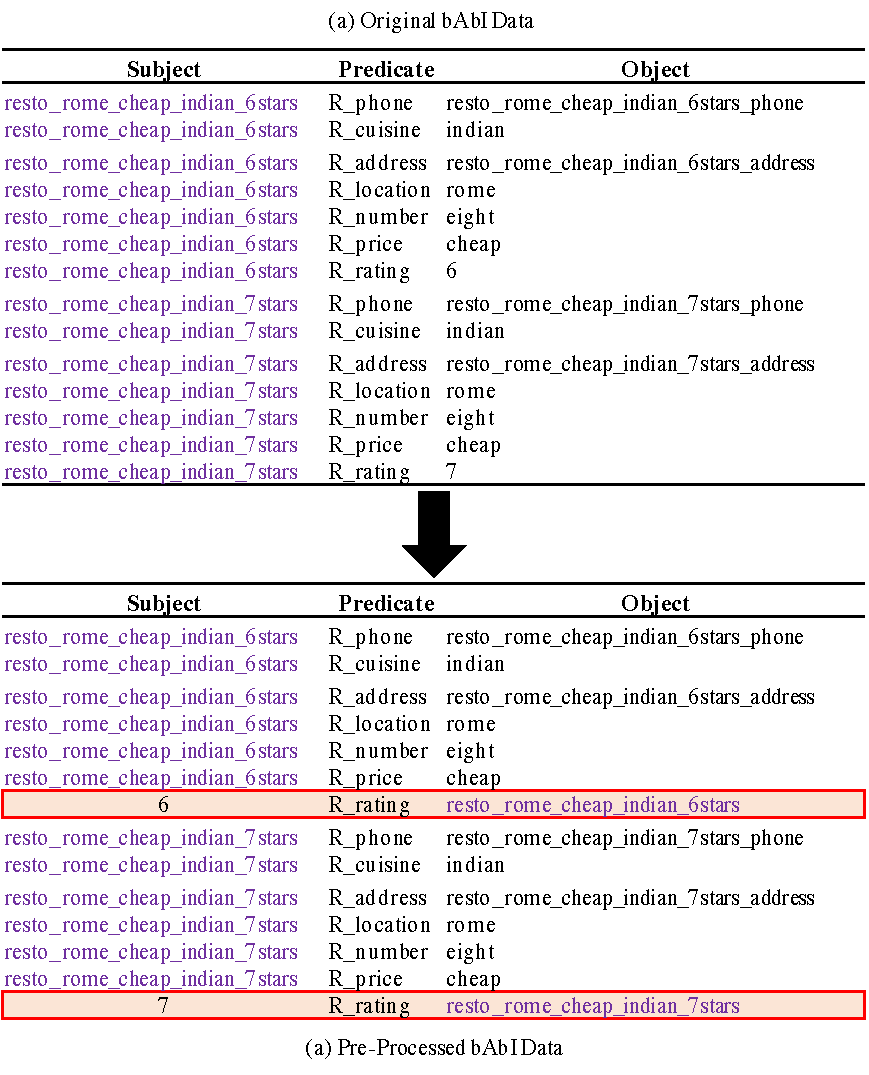
\includegraphics[width=0.8\textwidth]{assets/babi-preprocess.pdf}
\caption{Pre-processing of bAbI dialog data used in Mem2Seq paper}
\label{fig:prebabi}
\end{figure*}

\begin{figure*}[ht]
\centering
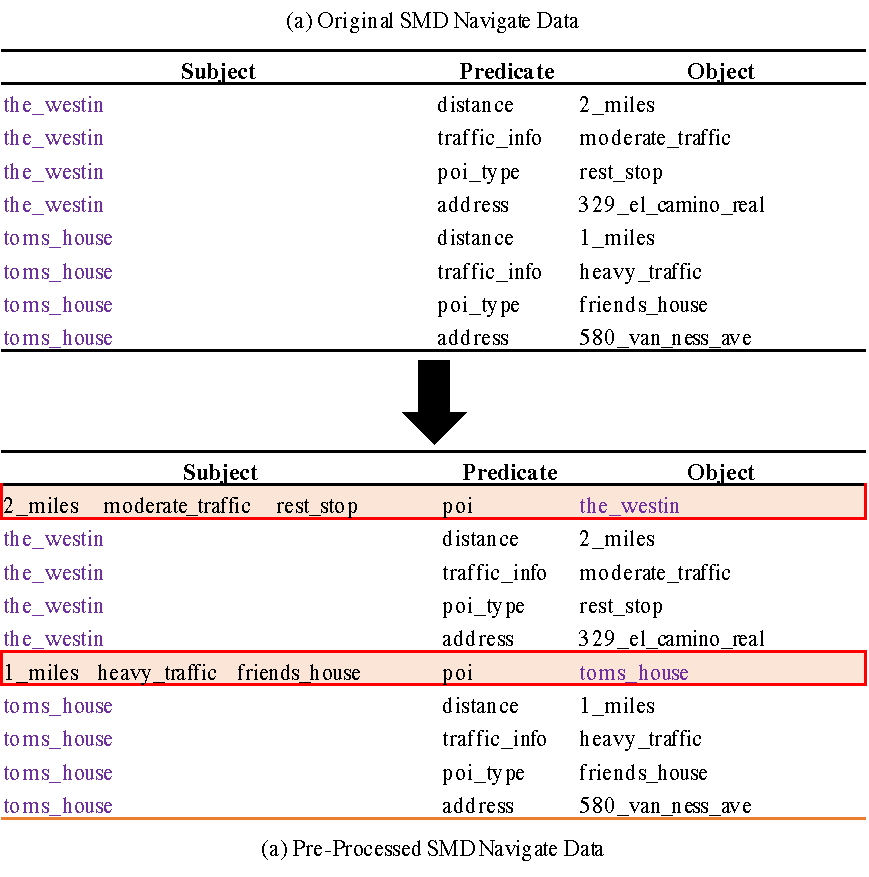
\includegraphics[width=0.8\textwidth]{assets/smd-preprocess.pdf}
\caption{Pre-processing of SMD Navigate data used in Mem2Seq paper}
\label{fig:presmd}
\end{figure*}

Mem2Seq paper used the following pre-processing on the data:
\begin{enumerate}
    \item The subject (restaurant name) and object (rating) positions of the rating KB tuples in bAbI dialogs are flipped, while the order remains the same for other tuples remains the same. This pre-processing is illustrated in Figure \ref{fig:prebabi}
    \item an extra fact was added to the navigation tasks in In-Car Assistant with all the properties (such as distance, address) combined together  as the subject and \textit{poi} as the object. This pre-processing is illustrated in Figure \ref{fig:presmd}
\end{enumerate}
The pre-processing has major impact on the performance of  Mem2Seq, as it can only copy objects of a KB tuple, while the subject and relation can never be copied.

\subsection{bAbI Dataset Faults}
\label{sec:fault}
The KB entities present in validation and non-OOV test sets for task 3 and 4 do not overlap with those in the train set. This effectively means that non-OOV and OOV test conditions are the same for tasks 3 and 4. This explains the low performance of baseline models on task 3 and 4 non-OOV test sets.

\section{AMT Setup}
\label{sec:amt_setup}
\begin{figure*}[h]
    \centering
    \subcaptionbox{\label{sfig:testa}}{
    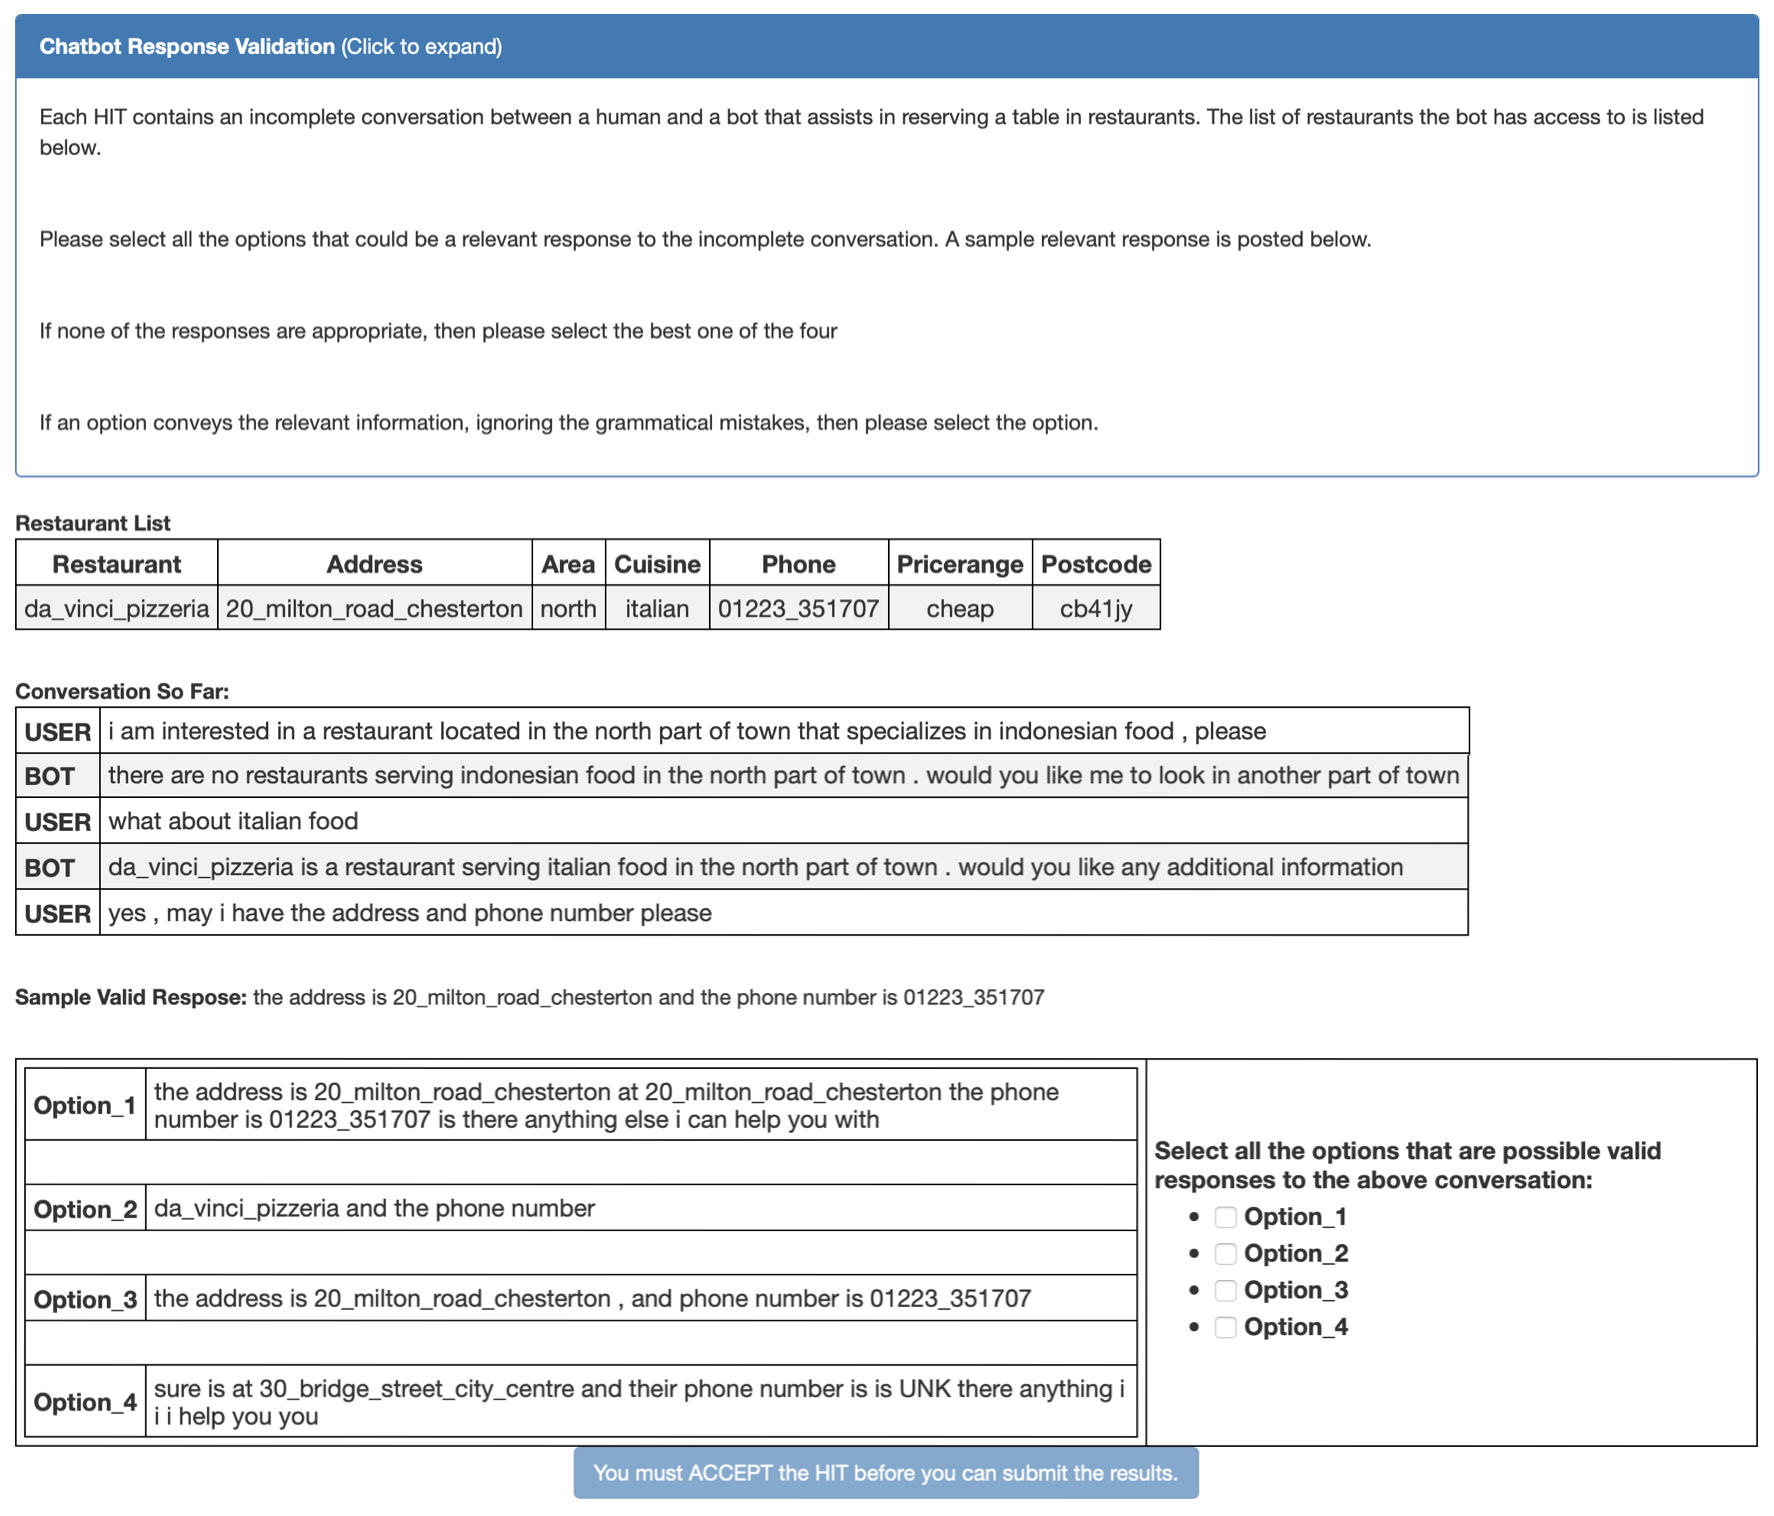
\includegraphics[width=0.9\textwidth]{assets/AMT_screen.png}}
    \subcaptionbox{\label{sfig:testb}}{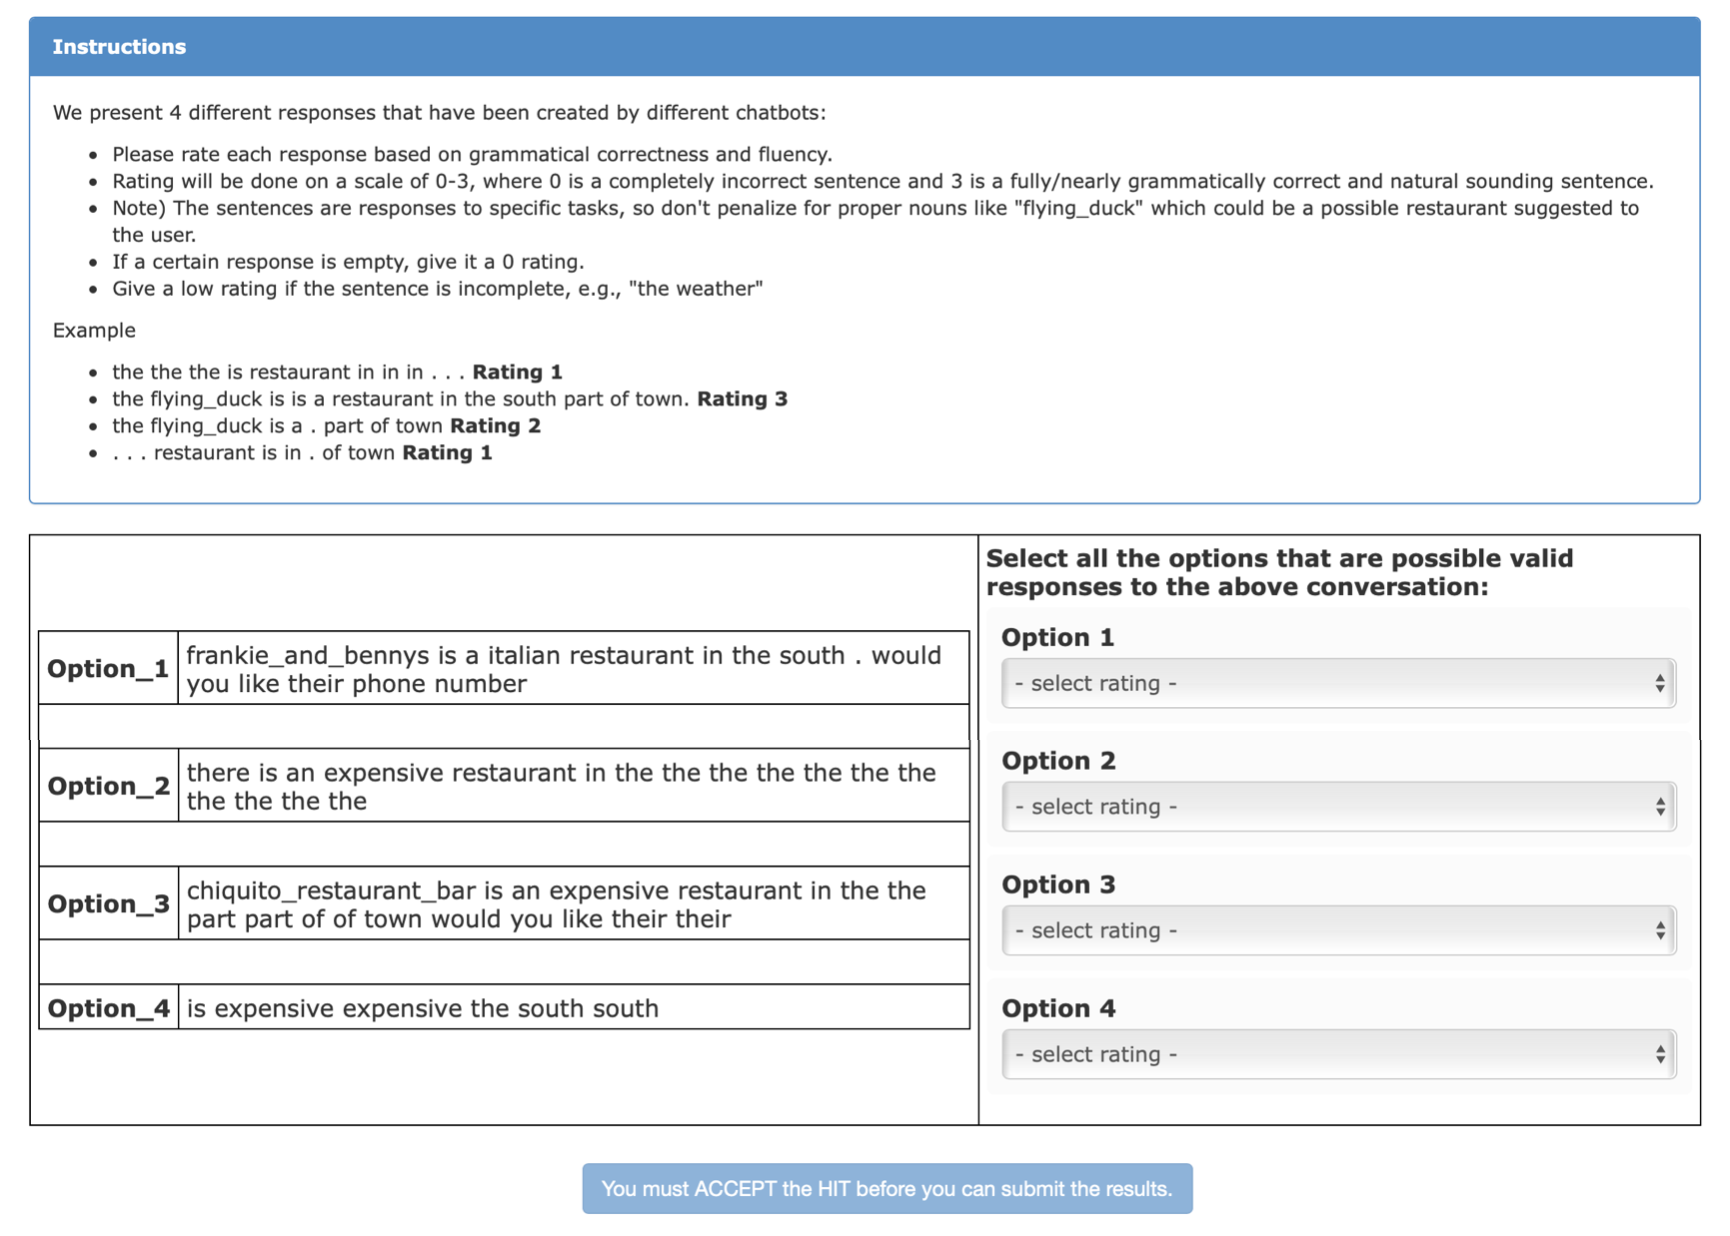
\includegraphics[width=0.9\textwidth]{assets/AMT_screen_grammar.png}}
    \caption{A sample HIT on Amazon Mechanical Turk to (a) validate useful responses based on the given dialog context, and (b) validate grammatical correctness of different responses on a scale of 0-3}
    \label{fig:amt_rel}
\end{figure*}

\noindent \textbf{Response Relevance Test} 
We show a sample of an Human Intelligence Task (HIT) on Amazon Mechanical Turk in Figure \ref{sfig:testa}. We randomize the responses generated by the three baseline models and \sys\ on the same dialog and ask the user to tick all those response options that seem to capture the relevant information of the given sample response. A total of 200 such annotations were collected for Camrest and SMD each.

\noindent \textbf{Response Grammar Test}
We show a sample of an Human Intelligence Task (HIT) on Amazon Mechanical Turk in Figure \ref{sfig:testb}. We randomize the responses generated by the three baseline models and \sys\ on the same dialog and ask the user to rate each response based on the grammatical correctness and natural flow of the sentence. The rating ranges from 0-3 where 0 being the worst and 3 being the best. Note) the sentences were not asked to be rated with respect to each other, but instead as individual occurrences. A total of 200 such annotations were collected for Camrest and SMD each.

\section{Multi-Hop vs 1-Hop Encoders}
Table \ref{tab:ablationhop} shows the performance of bAbI tasks and CamRest on two \sys\ encoder settings. Multi-hops in encoder helps in bAbI task 3 and 5, as they require inferencing over the KB tuples (sorting restaurants by rating) to recommend a restaurant. We also see substantial improvements on CamRest in both BLEU and entity F1 metric.

\begin{table*}
\centering
\footnotesize
\begin{tabular}{l|ccccc|ccccc|cc}
\toprule
   & \multicolumn{5}{c|}{\textbf{bAbI Dialog Tasks}} & \multicolumn{5}{c|}{\textbf{bAbI Dialog Tasks (OOV)}}  & \multicolumn{2}{c}{\textbf{CamRest}} \\ \cmidrule{2-6} \cmidrule{7-11} \cmidrule{12-13}
    & T1  & T2  & T3   & T4   & T5   & T1 & T2 & T3 & T4 & T5 & BLEU        & Ent. F1       \\ \midrule
\sys\ with 1-Hop Encoder & 100 & 100 & 92.3 & 100 & 90.5 & 100 & 100 & 91.4 & 100 & 89 & 10.5 & 36.9 \\
\sys\ with Multi-Hop Encoder & 100 & 100 & 95.2 & 100  & 97.3 & 100    & 100    & 95.7   & 100    & 91.7   & 15.2        & 43.1    
\\ \bottomrule
\end{tabular}
\caption{Ablation study: impact of hops in \sys\ encoder }
\label{tab:ablationhop}
\end{table*}